\section{Update phase}

  While the forward and backward pass perform cross--correlations and
  convolutions with a relatively large image with a small kernel
  producing another relatively large image, the cross--correlations
  performed during the update phase are performed on a large image
  with another large image resulting in a small image.

  The main difference between the cross--correlations performed during
  the fwd-bwd pass and the update phase is that

Similarly as in the fwd--bwd algorithm, our update phase algorithm
  consists of the following stack of primitives.

  Instead of computing
  \[
  \frac{\partial L}{\partial W_{j,i}} = \sum_{b=1}^B
  \frac{\partial L}{\partial I'_{b,j}}  \star I_{b,i}
  \]
  we compute
  \[
  \Bigg( \frac{\partial L}{\partial W_{j,i}} \Bigg)^T = \sum_{b=1}^B
  I_{b,i} \star \frac{\partial L}{\partial I'_{b,j}}
  \]

  That is the $GW^T$ tensor.

  In the update phase, each of the $F$ input images from the previous
  forward pass is cross--correlated with each of the $F'$ gradients
  with respect to the output obtained during the backward pass to
  produce $S^2$ gradients with respect to the kernel weights each of
  size $W_Z \times W_Y \times X$ -- the size of the kernel.  For
  simplicity, we will refer to the input images as simply ``images'',
  to the gradients with respect to the output as simply ``gradients'',
  and gradients with respect to the kernel weights as ``kernel
  gradients''.

  \begin{enumerate}
    \item {\bf Sub--kernel primitive} -- a primitive that computes a
      cross--correlation of each of $S$ images of size $R_Z \times R_Y
      \times (X + R_X - 1)$ with $S$ gradients of size $1 \times 1
      \times X$ to produce and accumulate the results of $S^2$ kernel
      gradients of size $R_Z \times R_X \times R_Y$.  As in the
      fwd--bwd case, this primitive is optimized for efficiently
      reusing the register file as well as $L1$ cache.
    \item {\bf Full kernel primitive} -- a primitive that computes
      cross--correlation of an arbitrary sized $S$ images with
      arbitrary sized $S$ gradients to produce $S^2$ kernel gradients.
    \item {\bf Sub--layer primitive} -- a primitive that computes
      $\alpha \times \beta \times S^2$ kernel gradients by
      cross--correlating each of $\alpha S$ images with $\beta S$
      gradients.
    \item {\bf Full layer primitive} -- parallelized primitive that
      divides the computation into a set of previous primitives and
      statically schedules execution.  As described below, this
      primitive might need to contain an extra parallelized reduction
      step, which is also statically scheduled.
  \end{enumerate}


  \begin{algorithm}
    {\footnotesize
      \begin{codebox}
        \Procname{$\proc{Update-Subtask} \langle R_x, R_y, R_z, Z, R_s \rangle(i,og,wg^T)$}
        \li \kw{simd register} $oreg[R_x][R_y][R_z][R_s]$
        \li \kw{simd register} $wreg$
        \li \For $s_0 \gets 0 \To S/R_s - 1$
        \li \Do $oreg[:][:][:][s_0R_s:s_0R_s+R_s-1][:] \gets$
        \li   \Do $\proc{LOAD}(wg^T[:][:][:][s_0R_s:s_0R_s+R_s-1][:])$
        \End
        \li \For $z_g \gets 0 \To Z-1$ \Comment Partially unrolled
        \li   \Do $wreg \gets \proc{LOAD}(og[1][1][z_g][:])$
        \li   \For $x \gets 0 \To R_x-1$ \Comment Fully unrolled
        \li   \Do \For $y \gets 0 \To R_y-1$  \Comment Fully unrolled
        \li   \Do \For $z \gets 0 \To R_z-1$  \Comment Fully unrolled
        \li   \Do \For $s_1 \gets 0 \To R_S-1$   \Comment Fully unrolled
        \li   \Do $oreg[x][y][z][s_0 \cdot R_s + s] \gets \proc{FMADD}($
        \li   \Do $wreg,$
        \li       $\proc{EXLOAD}(i[x][y][z+i][s_0 \cdot R_s + s]),$
        \li       $oreg[x][y][z][])$
        \End
        \End \li \kw{end for} $s$
        \End \li \kw{end for} $x$
        \End \li \kw{end for} $y$
        \End \li \kw{end for} $z$
        \End \li \kw{end for} $i$
        \li $wg^T[:][:][:][s_0R_s:s_0R_s+R_s-1][:] \gets$
        \li \Do $\proc{STORE}(oreg[:][:][:][s_0R_s:s_0R_s+R_s-1][:])$
        \End
        \End \li \kw{end for} $s_0$
      \end{codebox}
    \caption{Serial update subtask.}
    \label{alg:serial-update-subtask}
    }
  \end{algorithm}

  {\bf Sub--kernel primitive} \quad The lowest level primitive is
  shown in Algorithm~\ref{alg:serial-update-subtask}.  Following the
  same principles as in the fwd-bwd pass' sub--kernel primitive we
  vectorize the computation of $wg^T[r_x][r_y][r_z][f][f']$ computed
  via {\small
  \[
  \sum_{z}
  a[r_x][r_y][r_z+z][f] \cdot b[r_x][r_y][r_z][f']
  \]
  } such that the values of $wg^T[r_x][r_y][r_z][f][:]$ are computed
  via {\small
  \[
  \sum_{z}
  a[r_x][r_y][r_z+z][f] \cdot b[r_x][r_y][r_z][:]
  \]
  } Again, we recognize the reuse of $og[r_x][r_y][r_z][:]$ and
  re--order the loops appropriately.  In order to allow in--register
  computation, same constraints are imposed on $R_x \times R_y \times
  R_z \times R_s$ -- Maximal of $31$ for AVX512 and $8$ for SSE4, AVX
  and AVX2.  Additionally we allow only values for $R_s$ that divide
  $S$.  In order for the working set to fit inside the $L1$ cache, $Z$
  should be sufficiently small.  The number of bytes required for the
  working set equals $4S(R_xR_y+1)(R_z+Z-1)$.  For a given choice of
  $R_x, R_y$ and $R_z$, and given size of $L1$ cache, we
  conservatively choose $Z$ so that no more than half the cache is
  required for the working set.

   \begin{figure}
     \centering
     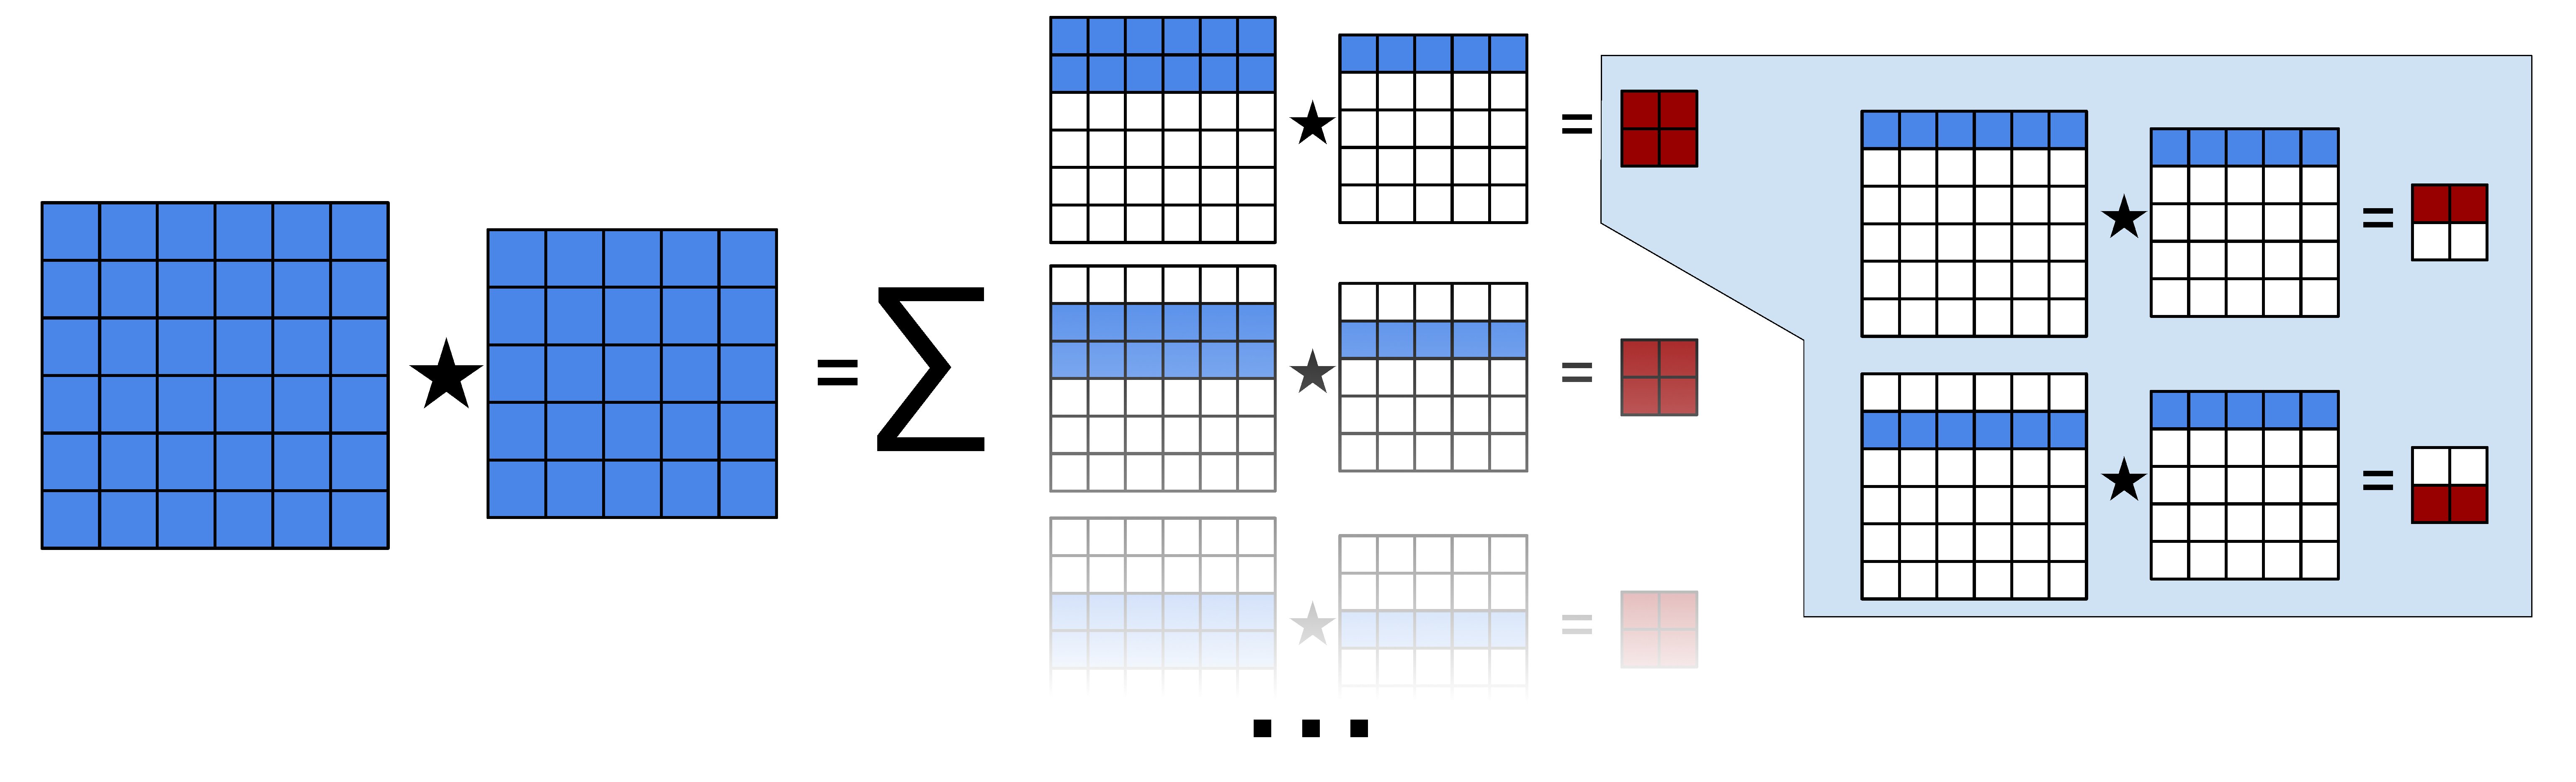
\includegraphics[width=0.99\linewidth]{fig/update2}
     \caption{An example of the {\bf full kernel primitive} and {\bf
         full gradient primitive} for the special case of $S=1$,...}
     \label{fig:conv-decomposition}
   \end{figure}

  {\bf Full kernel primitive} computes $S^2$ kernel gradients by
  cross--correlating each of $S$ images with $S$ gradients.  The
  computation is performed in two steps.  First, the gradients are
  split into sub--gradients of size $1 \times 1 \times Z$.  The result
  is then obtained as the sum of cross--correlations of each of the
  sub--gradients with an appropriate sub--image, as depicted on
  Fig~\ref{conv-decomposition} (middle column).  The
  cross--correlation of each sub--gradient is further split into
  sub--kernel primitives (right column on
  Fig.~\ref{conv-decomposition}.  We choose the $R_x, R_y, R_z$ and
  $R_s$ to maximize the register--file utilization, but subject to the
  limits described above.  Further, we require that $R_x, R_y$ and
  $R_z$ divide $K_x, K_y$ and $K_z$ respectively.  Note that this can
  always be accomplished be setting $R_x=R_y=R_z$ and $R_s=S$.
  However this choice might not be optimal.  For example, when $K_z=3$
  on AVX512 CPU, we could pick $R_s=8$ and $R_z=3$, which utilizes
  $24$ registers, which is better than choosing $R_z=1$ and
  $R_s=S=16$.  The optimal division is the one for which $R_x \times
  R_y \times R_z \times R_s$ is maximized.  When more combinations are
  possible, we prefer ones with large values of $R_s$, then $R_z$
  etc...  The value for $Z$ is then obtained using as described above.

  The computation is performed by iterating over the least significant
  dimension, then second least significant, etc..

  {\bf Sub--layer primitive} performs $\beta S \beta' S$
  cross--correlation.  Each of $\beta S$ input images is
  cross--correlated with each of $\beta'S$ output gradients to produce
  $\beta S \beta' S$ kernel gradients.  This primitive is designed for
  maximal reuse of higher levels of cache.  To achieve that, the
  computation is performed in the same fashion as in the fwd--bwd
  sub--layer primitive (Fig.~\ref{fig:full-exec}).

  {\bf Full layer primitive} \quad The main goal of the primitive is
  to parallelize the computation over $T$ available threads.  In
  contrast to the fwd--bwd full layer primitive where each thread can
  execute multiple sub--layer primitives, here we assign exactly one
  sub--layer primitive to each thread.  Each thread then executes the
  primitive on the subset of $B$ input--image output--gradient pairs.
